\documentclass[sans,mathserif,aspectratio=169, 10pt]{beamer}

\usepackage{booktabs}
\usepackage[spanish, mexico]{babel}
\selectlanguage{spanish}
\decimalpoint
\usepackage[utf8]{inputenc}
\usepackage{tikz}
\usepackage{fourier}
\newcommand{\quotes}[1]{``#1''}
\usepackage{epstopdf}
\usepackage{mathtools}
\DeclarePairedDelimiter{\ceil}{\lceil}{\rceil}
\usepackage{commath}
\usepackage{amsmath,tabularx}
\usepackage{listings}
\usepackage{xcolor}
\usepackage[edges]{forest}
\graphicspath{{Images/}}
\usepackage[mathscr]{euscript}
\newcommand{\overbar}[1]{\mkern 1.5mu\overline{\mkern-1.5mu#1\mkern-1.5mu}\mkern 1.5mu}
\newcommand*\mean[1]{\overbar{#1}}

\newcommand\Fontvi{\fontsize{9}{7.2}\selectfont}
\definecolor{foldercolor}{RGB}{124,166,198}

\tikzset{pics/folder/.style={code={%
    \node[inner sep=0pt, minimum size=#1](-foldericon){};
    \node[folder style, inner sep=0pt, minimum width=0.3*#1, minimum height=0.6*#1, above right, xshift=0.05*#1] at (-foldericon.west){};
    \node[folder style, inner sep=0pt, minimum size=#1] at (-foldericon.center){};}
    },
    pics/folder/.default={20pt},
    folder style/.style={draw=foldercolor!80!black,top color=foldercolor!40,bottom color=foldercolor}
}

\forestset{is file/.style={edge path'/.expanded={%
        ([xshift=\forestregister{folder indent}]!u.parent anchor) |- (.child anchor)},
        inner sep=1pt},
    this folder size/.style={edge path'/.expanded={%
        ([xshift=\forestregister{folder indent}]!u.parent anchor) |- (.child anchor) pic[solid]{folder=#1}}, inner xsep=0.6*#1},
    folder tree indent/.style={before computing xy={l=#1}},
    folder icons/.style={folder, this folder size=#1, folder tree indent=3*#1},
    folder icons/.default={12pt},
}

\colorlet{punct}{red!60!black}
\definecolor{background}{HTML}{EEEEEE}
\definecolor{delim}{RGB}{20,105,176}
\colorlet{numb}{magenta!60!black}

\lstdefinelanguage{json}{
    basicstyle=\normalfont\ttfamily\tiny,
    columns=flexible,
    keepspaces=true,
    frame=lines,
    backgroundcolor=\color{background}
}

\mode<presentation>

%Colors
\definecolor{steel}{RGB}{52,102,136}
\definecolor{moss}{RGB}{139,187,159}
\definecolor{burnt}{RGB}{187,102,65}
\definecolor{sandy}{RGB}{186, 168, 111}
\definecolor{RoyalBlue}{RGB}{0,35,102}
\definecolor{cream}{RGB}{254, 246, 235}
\definecolor{slate}{RGB}{82, 85, 100}
\definecolor{fall}{RGB}{194, 91, 86} % frame color
\definecolor{light}{RGB}{150, 192, 206}

%Structure
\usefonttheme{professionalfonts}
\hypersetup{colorlinks,linkcolor=fall!80,urlcolor=fall!80}
\setbeamercolor{local structure}{fg=fall}
\setbeamercolor{background canvas}{bg=cream}
\setbeamercolor{frametitle}{bg=fall,fg=cream}
\setbeamercolor{title}{fg=steel!115}
\setbeamercolor{author}{fg=fall}

\defbeamertemplate*{title page}{customized}[1][]
{\centering
  \fcolorbox{fall}{white}{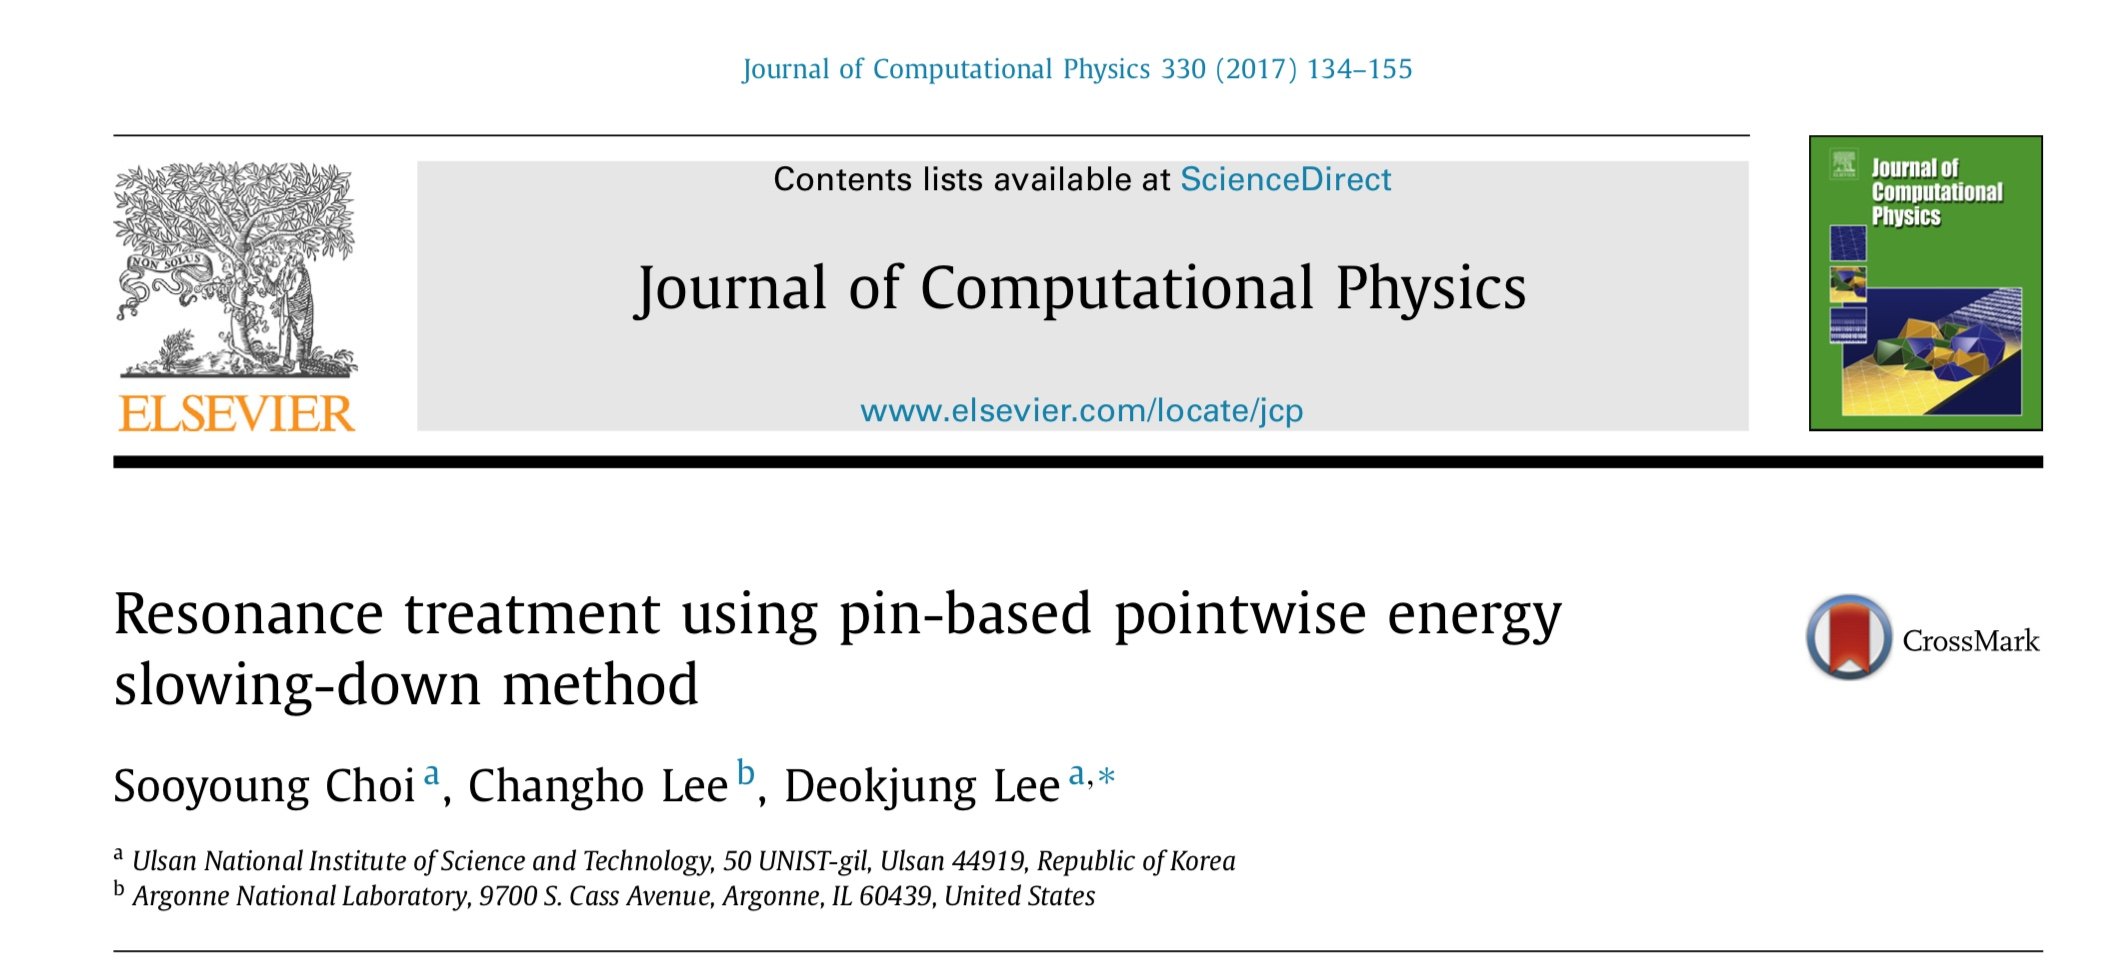
\includegraphics[width=0.80\linewidth]{cover.jpeg}}
  \vfill
  \usebeamerfont{author}\usebeamercolor[fg]{author}\insertauthor\par
  \vfill
  \usebeamerfont{institute}\insertinstitute\par
  \usebeamerfont{date}\insertdate\par
  \usebeamercolor[fg]{titlegraphic}\inserttitlegraphic
}

% Progressbar
\usepackage{tikz}
\usetikzlibrary{calc}

\makeatletter
\def\progressbar@progressbar{} % the progress bar
\newcount\progressbar@tmpcounta% auxiliary counter
\newcount\progressbar@tmpcountb% auxiliary counter
\newdimen\progressbar@pbht %progressbar height
\newdimen\progressbar@pbwd %progressbar width
\newdimen\progressbar@tmpdim % auxiliary dimension

\progressbar@pbwd=\paperwidth
\progressbar@pbht=2pt

\def\progressbar@progressbar{%

\progressbar@tmpcounta=\insertframenumber
\progressbar@tmpcountb=\inserttotalframenumber
\progressbar@tmpdim=\progressbar@pbwd
\multiply\progressbar@tmpdim by \progressbar@tmpcounta
\divide\progressbar@tmpdim by \progressbar@tmpcountb

  \begin{tikzpicture}[very thin]

  \shade[draw=steel!115,top color=steel,bottom color=steel,middle color=steel!115] %
    (0pt, 0pt) rectangle ++ (\progressbar@tmpdim, \progressbar@pbht);

  \end{tikzpicture}%
 }

\addtobeamertemplate{frametitle}{}
{%
  \vspace*{-16pt}
  \begin{beamercolorbox}[wd=\paperwidth,ht=1pt,dp=1pt]{}%
    \progressbar@progressbar%
  \end{beamercolorbox}%
}%
\makeatother

%Title
\title{Code Development Environment}
\subtitle{Experiences and Outlook}
\author[Guillermo Ibarra]{Guillermo Ibarra}
\date{Nuclear Engineering Research Seminar, April 28th, 2020}

\definecolor{keywords}{RGB}{255,0,90}
\definecolor{comments}{RGB}{0,0,113}
\definecolor{red}{RGB}{160,0,0}
\definecolor{green}{RGB}{0,150,0}

\setbeamercovered{transparent}
\setbeamercovered{%
  again covered={\opaqueness<1->{40}}}
\beamertemplatenavigationsymbolsempty


\begin{document}

%slide
\begin{frame}
\titlepage
\end{frame}

\begin{frame}{Introduction}
\begin{itemize}
\item Equivalence theory used resonance calculations.
\item Cao reported overestimation of multi-group $^{238}$U absorption XS (2015).
\item Present paper proposes a new resonance self-shielding method using a pointwise energy slowing-down solution (PSM). 
\end{itemize}
\end{frame}

\begin{frame}{Equivalence Theory}
Transport equation with collision probabilities:
\begin{equation}
\Sigma_{t,F}(E) \phi_F (E) V_F = P_{FF} V_F Q_{s,F} (E) + P_{MF}(E)V_M Q_{s,M} (E), \label{eq:basicCP}
\end{equation}
\pause
where
\begin{align}
Q_{s,F} (E) &= \sum_{r \in F} N^r \int_E^{E/\alpha^r} \sigma_s^r (E') \phi_F (E') \frac{1}{1-\alpha^r} \frac{dE'}{E'} \\
Q_{s,M} (E) &= \sum_{r \in M} N^r \int_E^{E/\alpha^r} \sigma_s^r (E') \phi_M (E') \frac{1}{1-\alpha^r} \frac{dE'}{E'} 
\end{align}
\end{frame}

\begin{frame}{Scattering Source}{IR approximation}
\begin{align}
 \int_E^{E/\alpha^r} \sigma_s^r (E') \phi_F (E') \frac{1}{1-\alpha^r} \frac{dE'}{E'} &\approx \lambda^r \sigma_p^r \frac{1}{E} + (1-\lambda^r) \sigma_s^r (E) \phi_F (E), \\
\int_E^{E/\alpha^r} \sigma_s^r (E') \phi_M (E') \frac{1}{1-\alpha^r} \frac{dE'}{E'} &\approx \lambda^r \sigma_p^r \frac{1}{E}
\end{align}
\end{frame}

\begin{frame}{Updated Collision Probabilities}
Rewriting Eq. \ref{eq:basicCP} using the approximate scattering source and a reciprocity theorem:
\begin{equation}
\Sigma_{t,F}(E) \phi_F (E) V_F = P_{FF} \left[\lambda_F \Sigma_{p,F} \frac{1}{E} + (1-\lambda_F) \Sigma_{s,F} (E) \phi_F (E)  \right]
+ P_{FM} (E) \Sigma_{t,F} (E) V_F \frac{1}{E},
\end{equation}
\pause
where $\lambda_X \Sigma_{p,X} = \sum_{r \in X} \lambda^r N^r \sigma_p^r$, ($X=F$ or $M$); and the reciprocity theorem: 
\begin{equation}
P_{FM} (E) \Sigma_{t,F} (E) V_F = P_{MF} (E) \Sigma_{t,M} V_M \approx P_{MF} (E) \lambda_M \Sigma_{p,M} V_M.
\end{equation}
\pause
Then, fuel-to-fuel collision probability is approximated by rational equation:
\begin{equation}
P_{FF} (E) = 1 - P_{FM} (E) = \sum_{n=1}^N \frac{\beta_n \Sigma_{t,F} (E)}{\Sigma_{t,F} (E) + \alpha_n \Sigma_e},
\end{equation}
\end{frame}

\begin{frame}{Total Flux}
Using a multi-term rational approximation, total flux is formulated as a linear combination:
\begin{equation}
\phi_F (E) = \sum_{n=1}^N \beta_n \phi_{F,n} (E) = \sum_{n=1}^N \beta_n \frac{\lambda_F \Sigma_{p,F} + \alpha_n \Sigma_e}{\Sigma_{a,F} (E) + \lambda_F \Sigma_{rs,F} (E) + \lambda_F \Sigma_{p,F} + \alpha_n \Sigma_e} \frac{1}{E},
\end{equation}
\pause
Dividing by $N^r$
\begin{equation}
\phi_F (E) = \sum_{n=1}^N \beta_n \phi_{F,n} (E) = \sum_{n=1}^N \beta_n \frac{\sigma_{b,n}^r}{\sigma_{a}^r (E) + \lambda^r \sigma_{rs}^r (E) + \sigma_{b,n}^r} \frac{1}{E},
\end{equation}
\pause
with the background XS:
\begin{equation}
\sigma_{b,n}^r = \frac{1}{N^r} (\lambda_F \Sigma_{p,F} + \alpha \Sigma_e).
\end{equation}
\end{frame}

\begin{frame}{Lethargy Form}
\Fontvi
\begin{equation}
\phi_F (u) = \sum_{n=1}^N \beta_n \phi_{F,n} (u) = \sum_{n=1}^N \beta_n \frac{\sigma_{b,n}^r}{\sigma_a^r(u) + \lambda_{rs}^r(u) + \sigma_{b.n}^r}
\end{equation}
Multi-group XS definition:
\begin{align}
\sigma_{x,g} &= \frac{\int_{\Delta u_g} \sigma_x^r (u) \phi_F (u)du}{\int_{\Delta u_g} \phi_F (u)du} = \frac{\int_{\Delta u_g} \sigma_x^r (u) \sum_{n=1}^N \beta_n \frac{\sigma_{b.n}}{\sigma_a^r (u) + \sigma_{b.n}} du}{\int_{\Delta u_g} \sum_{n=1}^N \beta_n \frac{\sigma_{b.n}}{\sigma_a^r (u) + \sigma_{b.n}} du} \nonumber \\
&= \frac{\sum_{n=1}^N \beta_n \int_{\Delta u_g} \sigma_x^r (u) \frac{\sigma_{b.n}}{\sigma_a^r (u) + \sigma_{b.n}} du}{\sum_{n=1}^N \beta_n \int_{\Delta u_g} \frac{\sigma_{b.n}}{\sigma_a^r (u) + \sigma_{b.n}} du} =  \frac{\sum_{n=1}^N \beta_{n,g} \sigma_{x,n,g}^r (u) \phi_{n,g}}{\sum_{n=1}^N \beta_{n,g} \phi_{n,g}} 
\end{align}
\pause
where,
\begin{align}
\sigma_{x,n,g}^r &= \sigma_{x,g}^r \left(\sigma_{b,n,g}^r \right), \quad x = a,s,f, \\
\phi_{n,g} &= \phi_g \left(\sigma_{b,n,g}^r \right) = \frac{\sigma_{b,n,g}^r}{\sigma_{a,n,g}^r + \sigma_{b,n,g}^r} \\
\sigma_{b,n,g}^r &= \frac{1}{N^r} \left(\sum_r \lambda_g^r N^r \sigma_p^r + \alpha_{n,g} \Sigma_e  \right)
\end{align}
\end{frame}

\begin{frame}{Resonance Integral Form}
\begin{equation}
\sigma_{x,g}^r = \frac{\sum_{n=1}^N \beta_{n,g} RI_{x,n,g}^r}{1 - \sum_{n=1}^N \beta_{n,g} \frac{RI_{a,n,g}^r}{\sigma_{b,n,g}^r}},
\end{equation}
\pause 
where 
\begin{equation}
RI_{x,n,g}^r = \frac{\int_{\Delta u_g} \sigma_x^r (u) \phi_{F,n} (u) du}{\int_{\Delta u_g} du} = RI_{x,n}^r \left( \sigma_{b,n,g}^r \right) = \sigma_{x,n,g}^r \phi_{n,g}.
\end{equation}
\end{frame}

\begin{frame}{Modified Forms of Equivalence Theory}{WIMS}
\begin{equation}
\sigma_{x,g}^r = \frac{\sum_{n=1}^N \beta_{n,g} RI_{x,n,g}^r}{1 - \sum_{n=1}^N \beta_{n,g} \frac{\lambda RI_{rs,n,g}^r + RI_{a,n,g}^r}{\sigma_{b,n,g}^r}},
\end{equation}
\end{frame}

\begin{frame}{Modified Forms of Equivalence Theory}{Yamamoto}
\begin{align}
\tilde{\sigma}_{a,g}^r \sum_{n=1}^N \beta_{n,g} \frac{\sigma_{b,n,g}^r}{\tilde{\sigma}_{a,g}^r + \sigma_{b,n,g}^r} &= \sum_n^N  \beta_n \frac{\sigma_{a,n,g}^r\sigma_{b,n,g}^r}{\sigma_{a,n,g}^r + \sigma_{b,n,g}^r} , \\
\sigma_{x,g}^r &= \frac{\sum_{n=1} \beta_{n,g} \sigma_{x,n,g}^r \frac{\sigma_{b,n,g}^r}{\sigma_{a,n,g}^r + \sigma_{b,n,g}^r}}{\sum_{n=1}^N \beta_{n,g} \frac{\sigma_{b,n,g}^r}{\tilde{\sigma}_{a,g}^r + \sigma_{b,n,g}^r}}
\end{align}
\end{frame}

\begin{frame}{Modified Forms of Equivalence Theory}{Cao}
\begin{equation}
\sigma_{x,g}^r = \frac{\sum_{n=1} \beta_{n,g} \sigma_{x,n,g}^r \phi_{n,g}^{SD}}{\sum_{n=1}^N \beta_{n,g} \phi_{n,g}^{SD}}
\end{equation}
\end{frame}

\begin{frame}{Numerical Test with Equivalence Theory}
\centering
\fcolorbox{fall}{white}{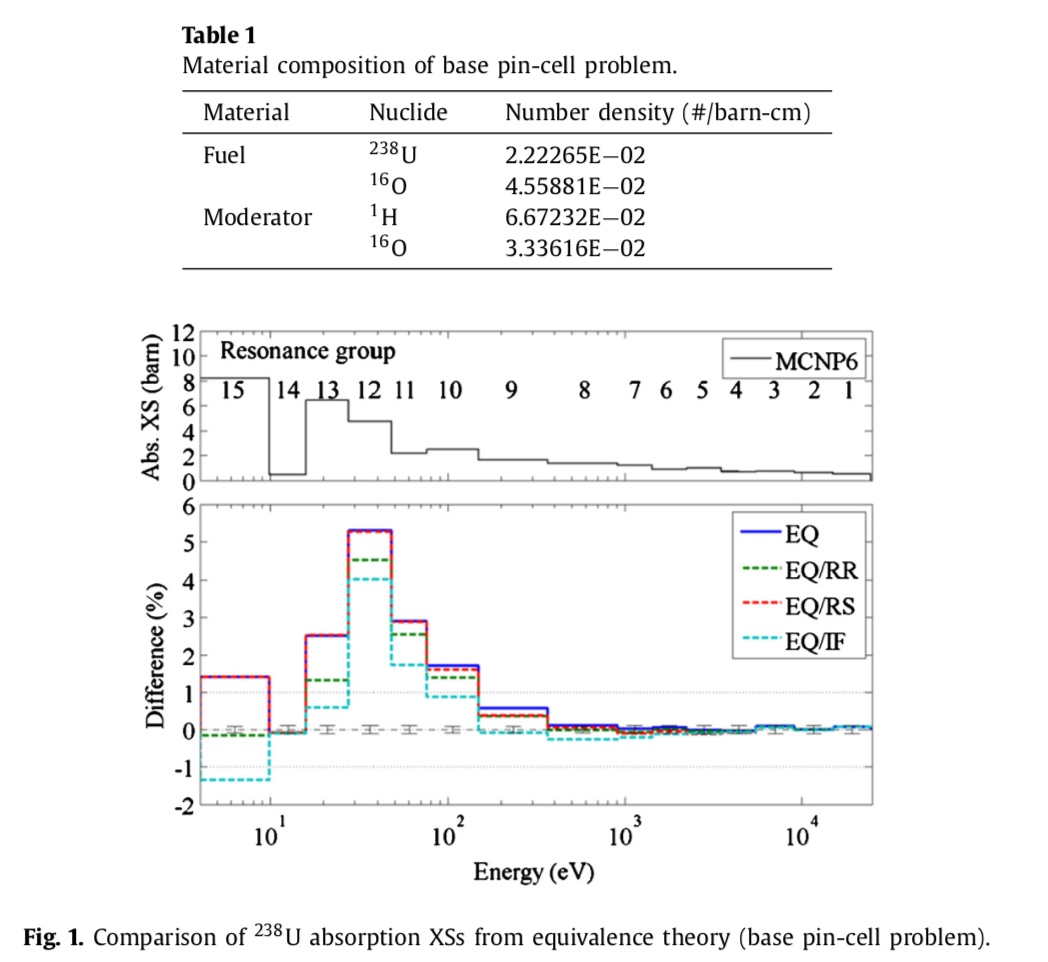
\includegraphics[width=0.50\linewidth]{fig1-tab1.jpeg}}
\end{frame}

\begin{frame}{Pointwise Energy Approach}
\begin{equation}
\Sigma_{t,F} (u) \phi_F (u) = P_{FF} (u) Q_{s,F} + P_{FM} (u) \Sigma_{t,F} (u)
\end{equation}
\pause
Flux specified as a rational approximation:
\begin{equation}
\phi_F (u) = \sum_{n=1}^N \beta_n \frac{Q_{s,F}(u) + \alpha_n \Sigma_e}{\Sigma_{t,F} (U) + \alpha_n \Sigma_e}
\end{equation}
\pause
Assuming that total flux is a linear combination and the IR approximation:
\begin{equation}
\phi_F (u) = \sum_{n=1}^N \beta_n \frac{\lambda \Sigma_{p,F} + \alpha_n \Sigma_e}{\Sigma_{t,F} (U) + \alpha_n \Sigma_e} = \sum_{n=1}^N \beta_n \phi_{F,n} (u)
\end{equation}
\end{frame}

\begin{frame}{Pointwise Energy Approach}{separated fluxes}
\begin{align}
&\Sigma_{t,F} (u) \phi_{F,n} (u) = \frac{\Sigma_{t,F} (u)}{\Sigma_{t,F} (u) + \alpha_n \Sigma_e} Q_{s,F,n} (u) + \left( 1 - \frac{\Sigma_{t,F} (u)}{\Sigma_{t,F} (u) + \alpha_n \Sigma_e} \right), \quad n = 1, \dots, N, \\
&\sigma_{x,g}^r = \frac{\int_{\Delta u_g} \sigma_x^r (u) \sum_{n=1}^N \beta_n \phi_{F,n} (u) du}{\int_{\Delta u_g}  \sum_{n=1}^N \beta_n \phi_{F,n} (u) du},
\end{align}
where
\begin{equation}
Q_{s,F,n} (E) = \sum_{r \in F} N^r \int_E^{E/\alpha^r} \sigma_s^r (E') \phi_{F,n} (E') \frac{1}{1-\alpha^r} \frac{dE'}{E'}
\end{equation}
\end{frame}

\begin{frame}{Pointwise Energy Approach}{separated fluxes}
\begin{align}
&\Sigma_{t,F} (u) \phi_F (u) = \sum_{n=1}^N \beta_n \frac{\Sigma_{t,F}(u)}{\Sigma_{t,F}(u) + \alpha_n \Sigma_e} Q_{s,F} (u) + \left( 1- \sum_{n=1}^N \beta_n \frac{\Sigma_{t,F}(u)}{\Sigma_{t,F}(u) + \alpha_n \Sigma_e} \right) \Sigma_{t,F} (u) \\
&\sigma_{x,g}^r = \frac{\int_{\Delta u_g} \sigma_x^r (u) \phi_F (u) du}{\int_{\Delta u_g} \phi_F (u) du}
\end{align}
Difference between fluxes:
\begin{equation}
\phi_F^S (u) - \phi_F^C (u) = \sum_{n=1}^N \beta_n \frac{Q_{F,n} (u) - Q_F (u)}{\Sigma_{t,F} (u) + \alpha_n \Sigma_e} \ne 0
\end{equation}
\end{frame}

\begin{frame}{Numerical Test with Pointwise Energy Approach}
\centering
\fcolorbox{fall}{white}{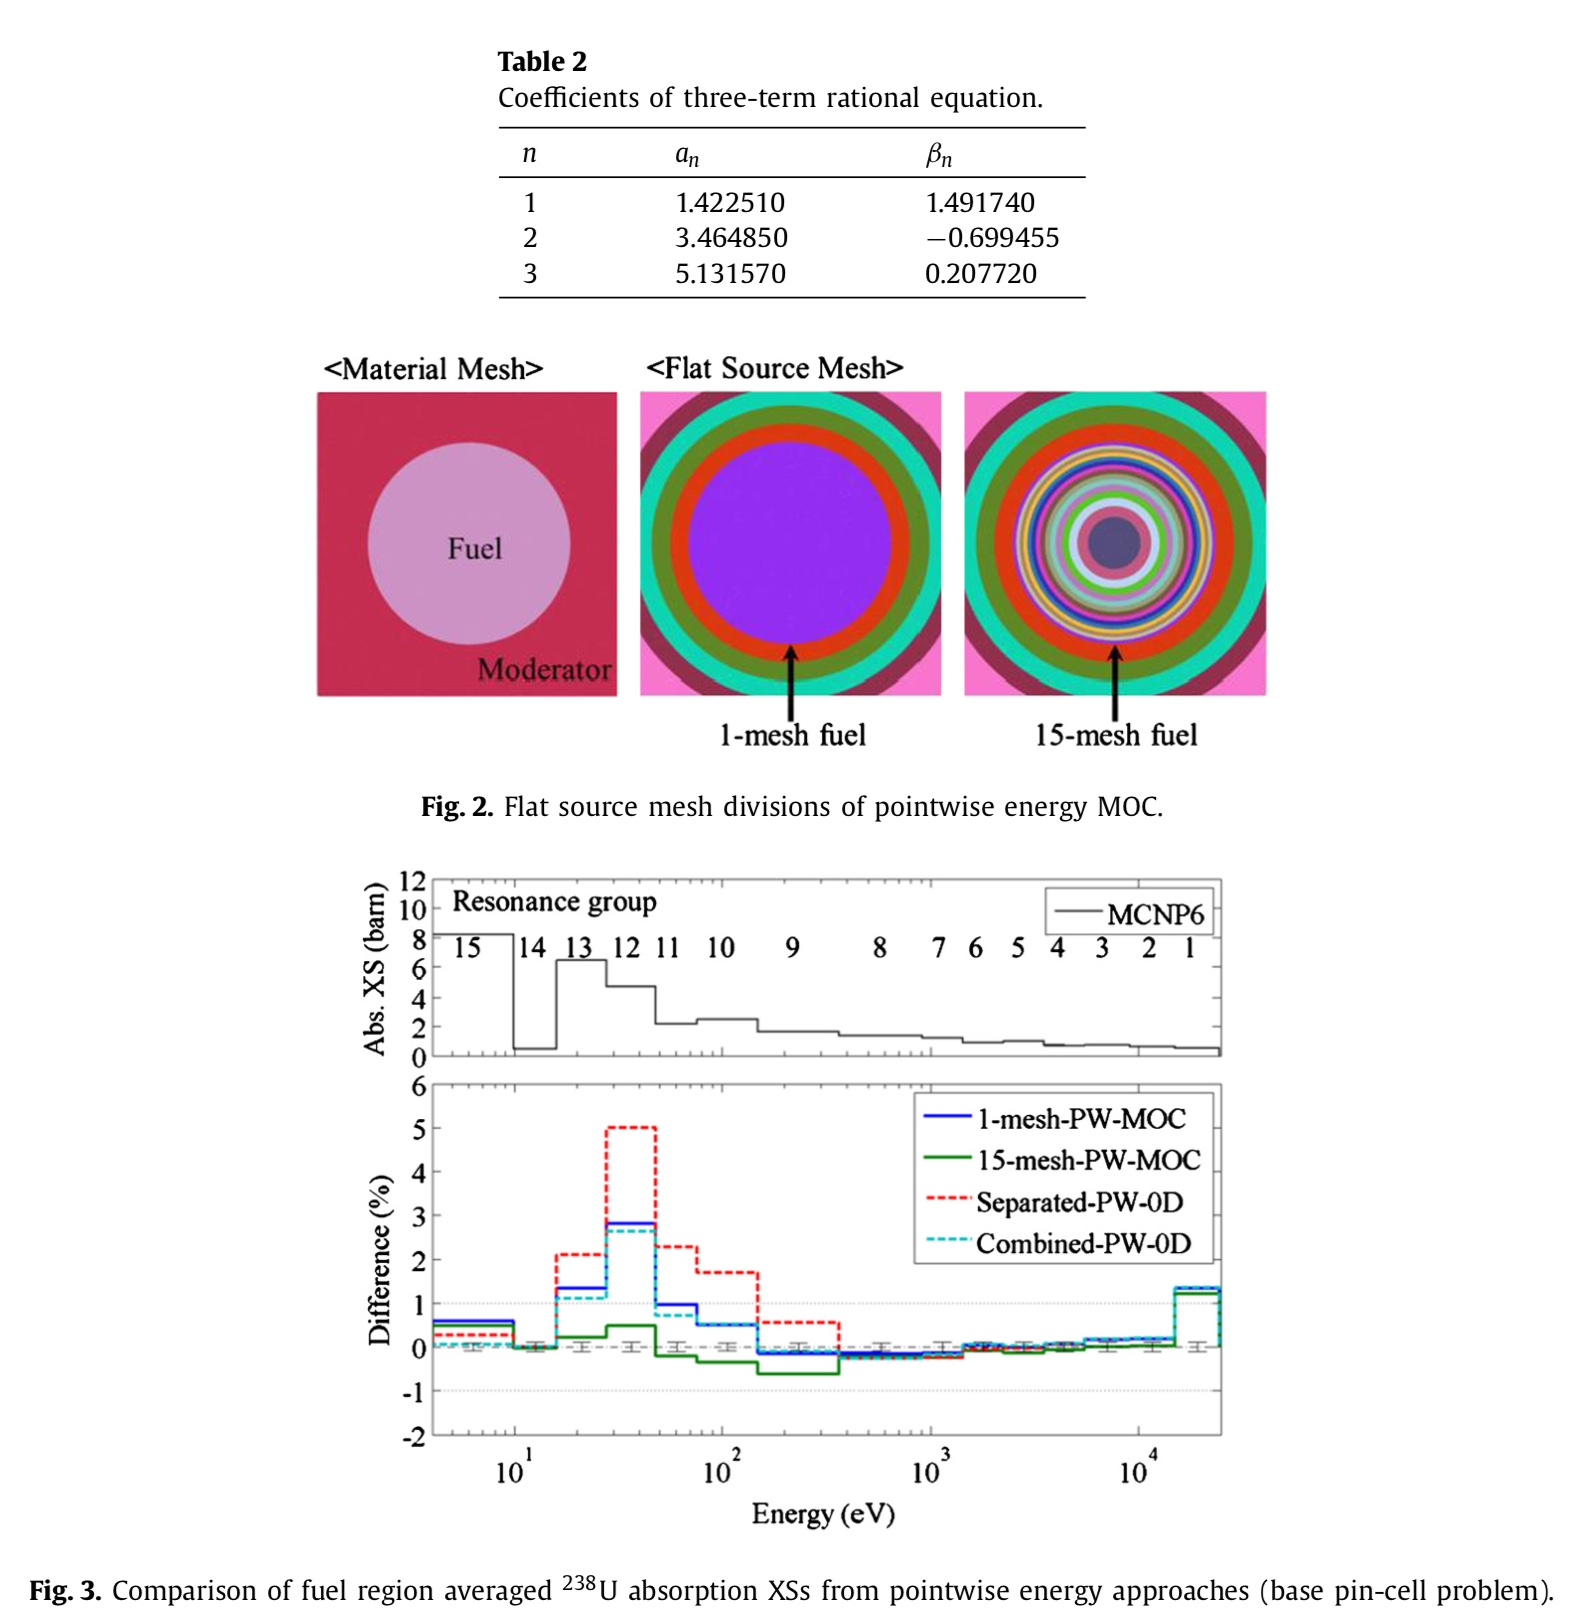
\includegraphics[width=0.50\linewidth]{tab2-fig2-3.jpeg}}
\end{frame}

\begin{frame}{Numerical Test with Pointwise Energy Approach}{Collision Probability}
\centering
\fcolorbox{fall}{white}{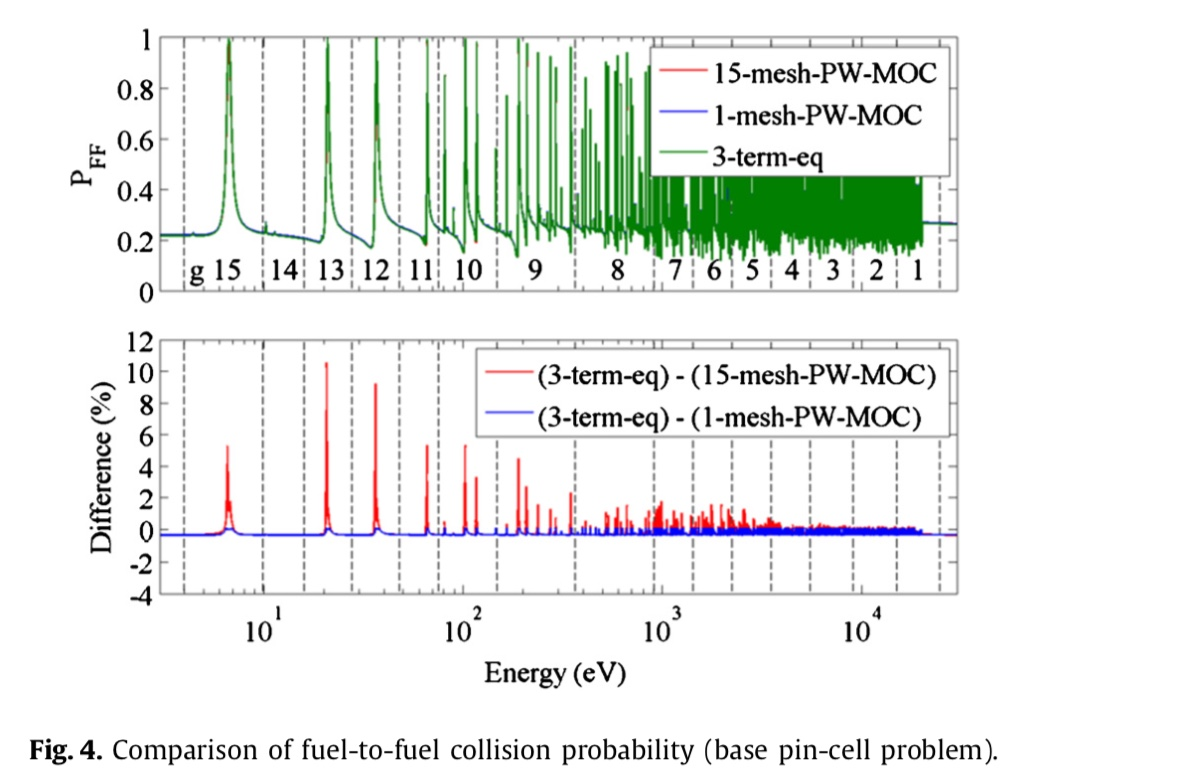
\includegraphics[width=0.75\linewidth]{fig4.jpeg}}
\end{frame}

\begin{frame}{Numerical Test Without Resonance Scattering Cross Section}
\centering
\fcolorbox{fall}{white}{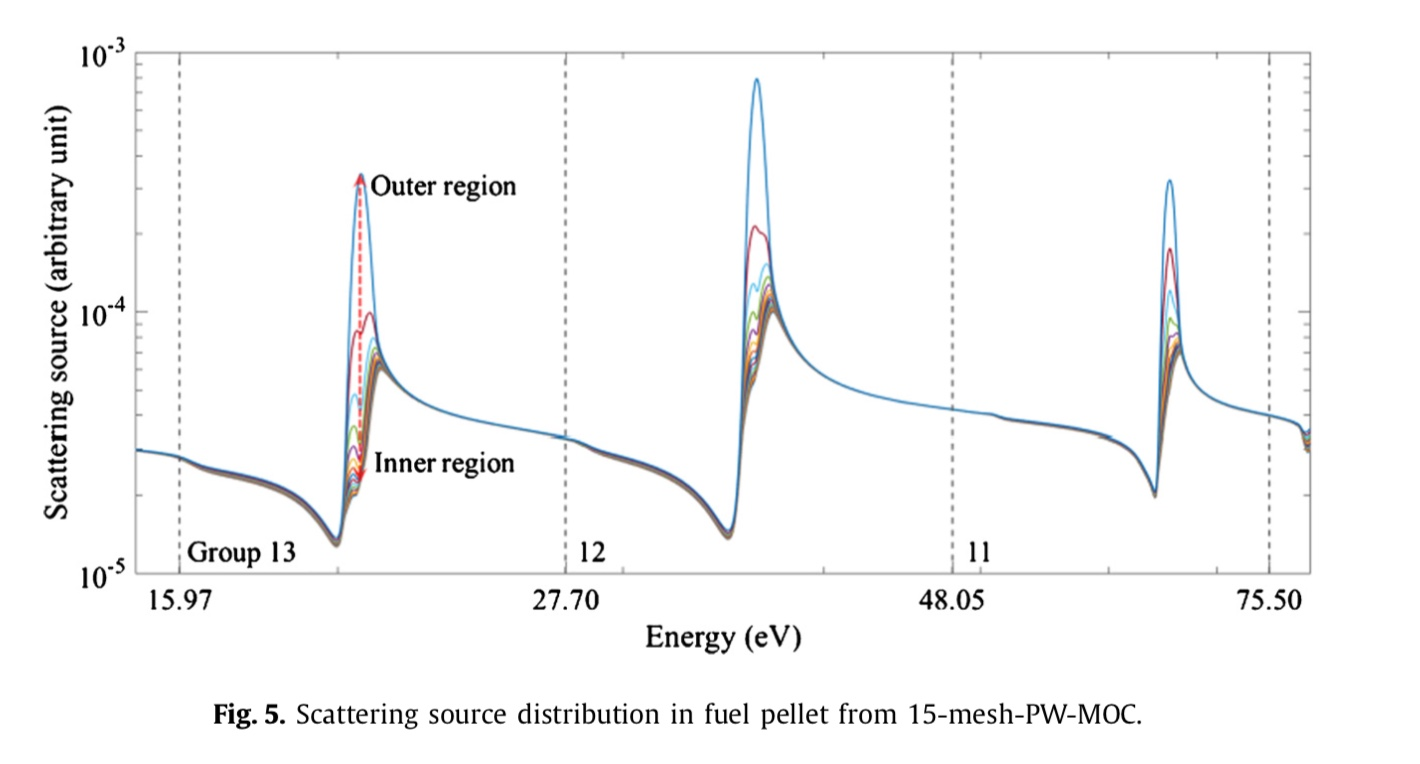
\includegraphics[width=0.75\linewidth]{fig5.jpeg}}
\end{frame}

\begin{frame}{Numerical Test Without Resonance Scattering Cross Section}
\centering
\fcolorbox{fall}{white}{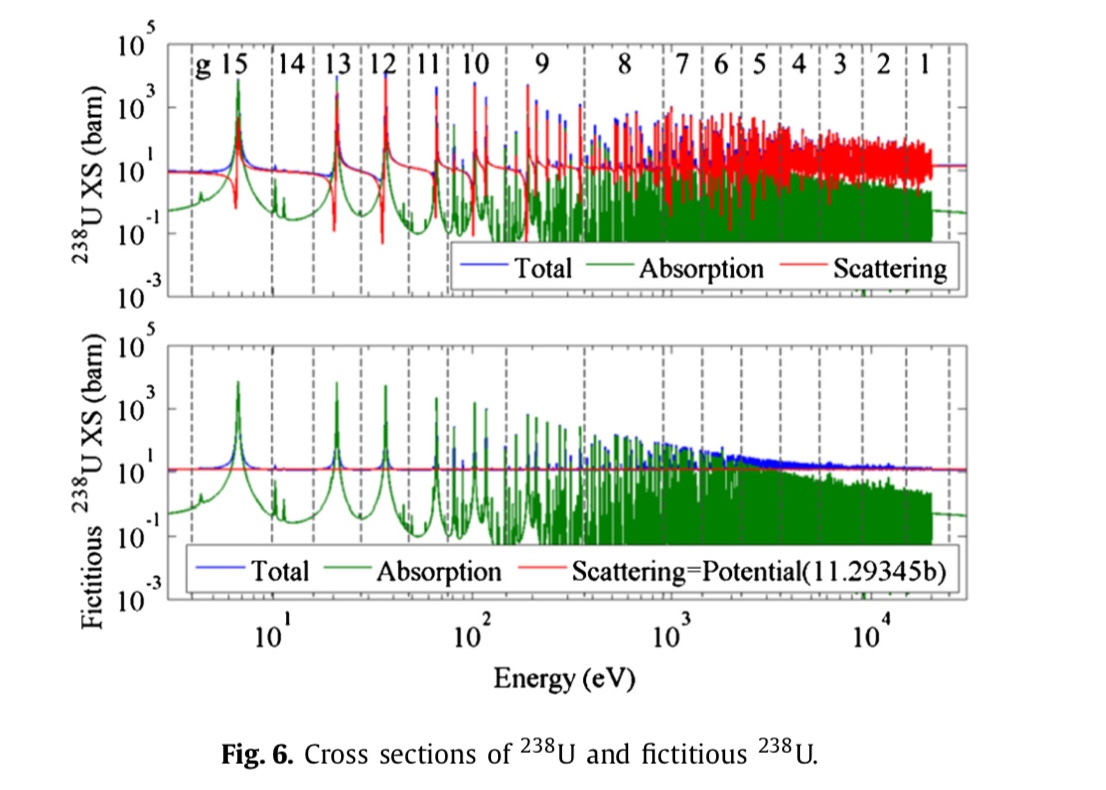
\includegraphics[width=0.70\linewidth]{fig6.jpeg}}
\end{frame}

\begin{frame}{Numerical Test Without Resonance Scattering Cross Section}
\centering
\fcolorbox{fall}{white}{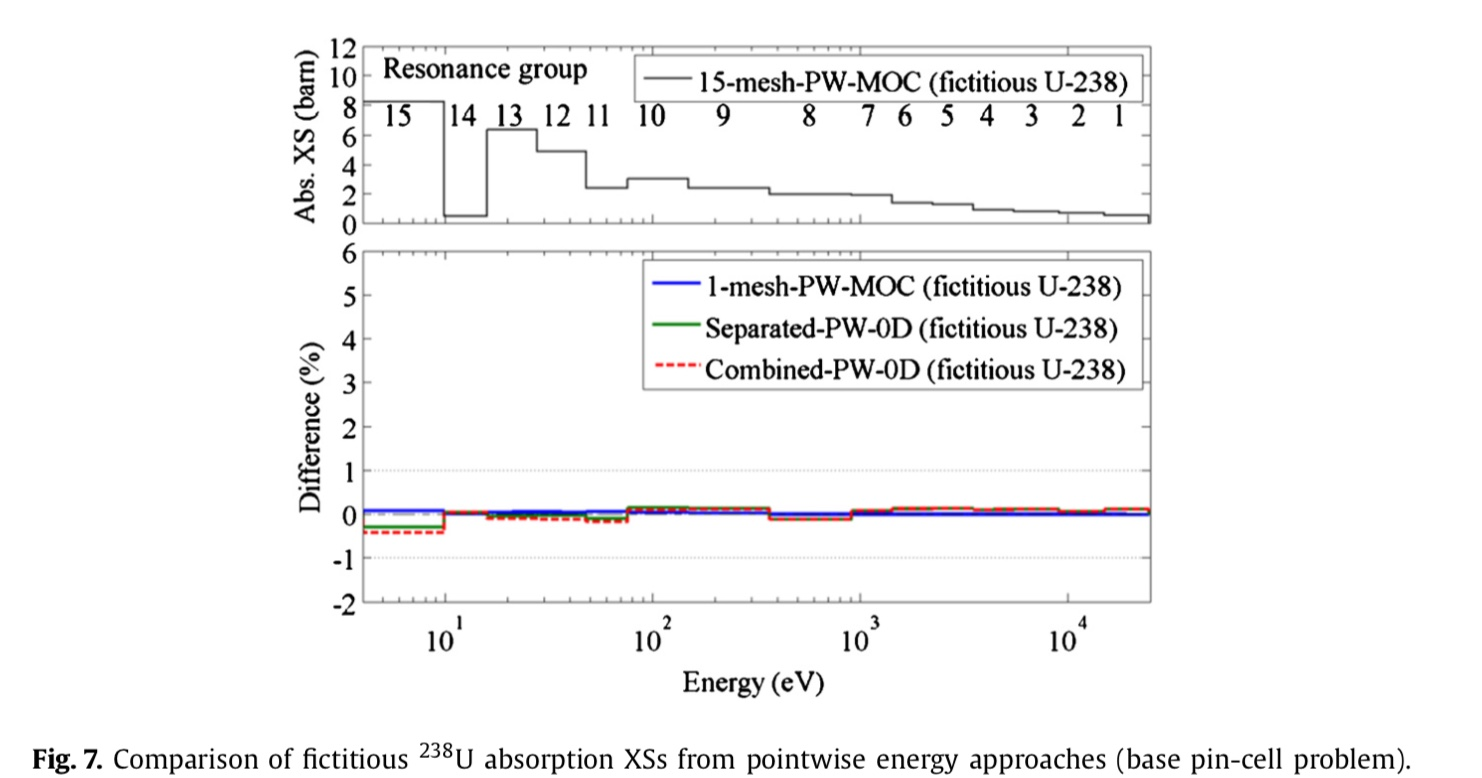
\includegraphics[width=0.75\linewidth]{fig7.jpeg}}
\end{frame}

\begin{frame}{New Resonance Self-Shielding Method}
\begin{itemize}
\item Comteporary spatially dependent methods
	\begin{itemize}
	\item SDDM
	\item ESSM
	\end{itemize}
\item Pin-based pointwise energy slowing-down method (PSM)
\end{itemize}
\end{frame}

\begin{frame}{PSM Collision Probability}
\centering
\fcolorbox{fall}{white}{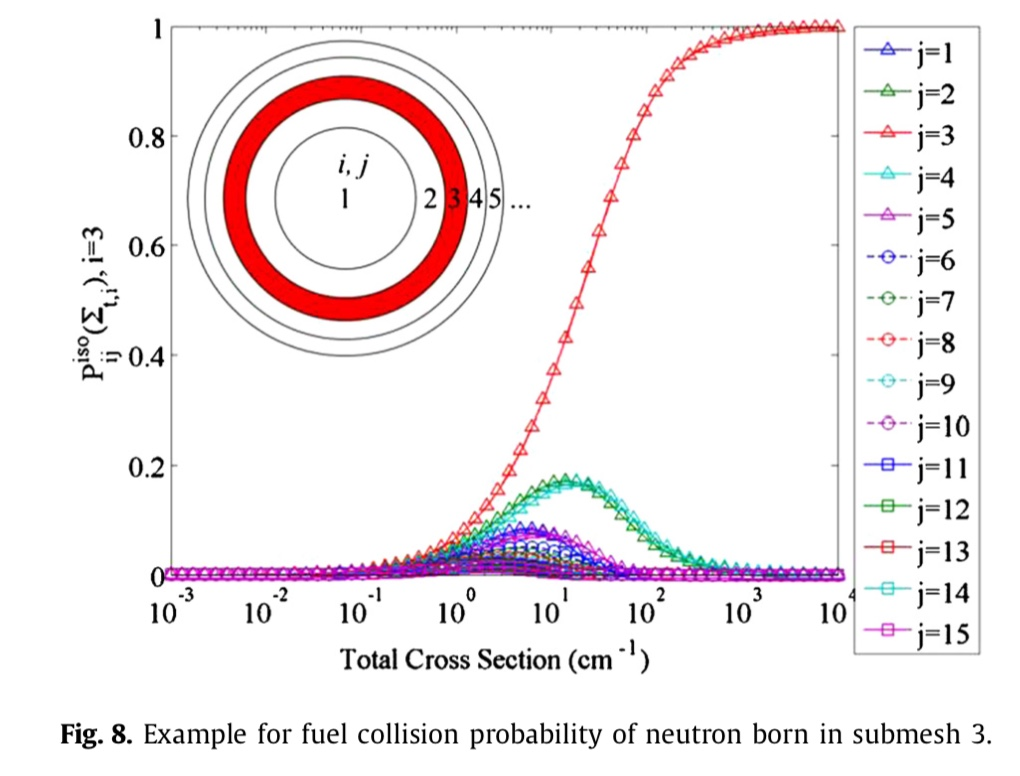
\includegraphics[width=0.65\linewidth]{fig8.jpeg}}
\end{frame}

\begin{frame}{PSM Escape Probability}
\centering
\fcolorbox{fall}{white}{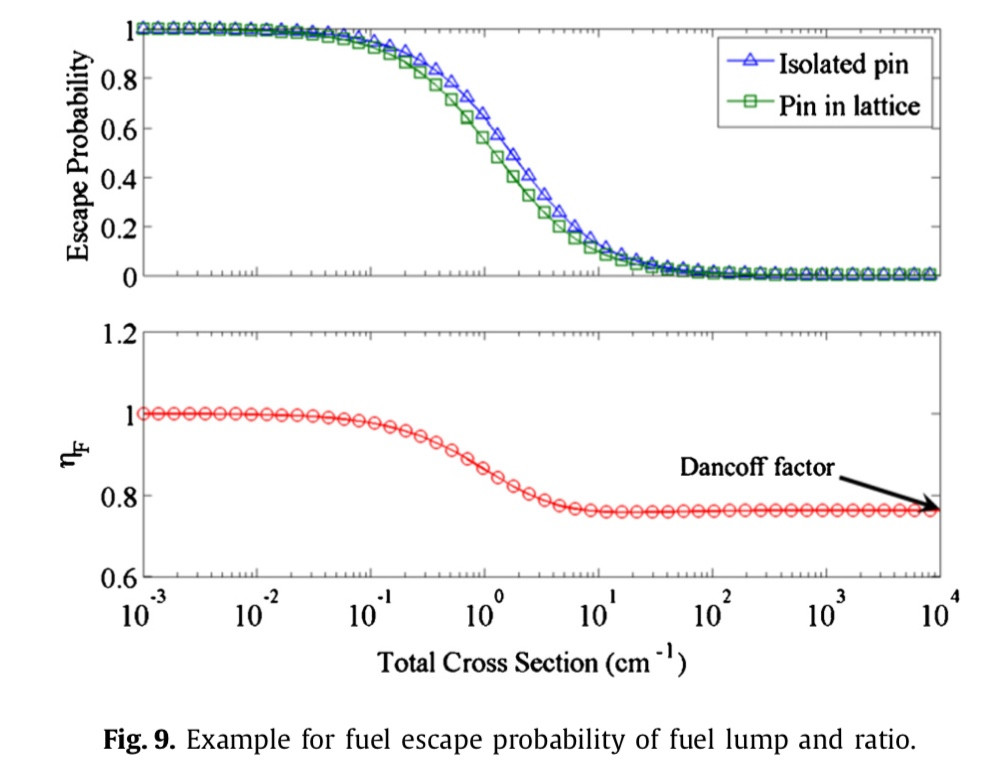
\includegraphics[width=0.65\linewidth]{fig9.jpeg}}
\end{frame}

\begin{frame}{PSM Calculation Flowchart}
\centering
\fcolorbox{fall}{white}{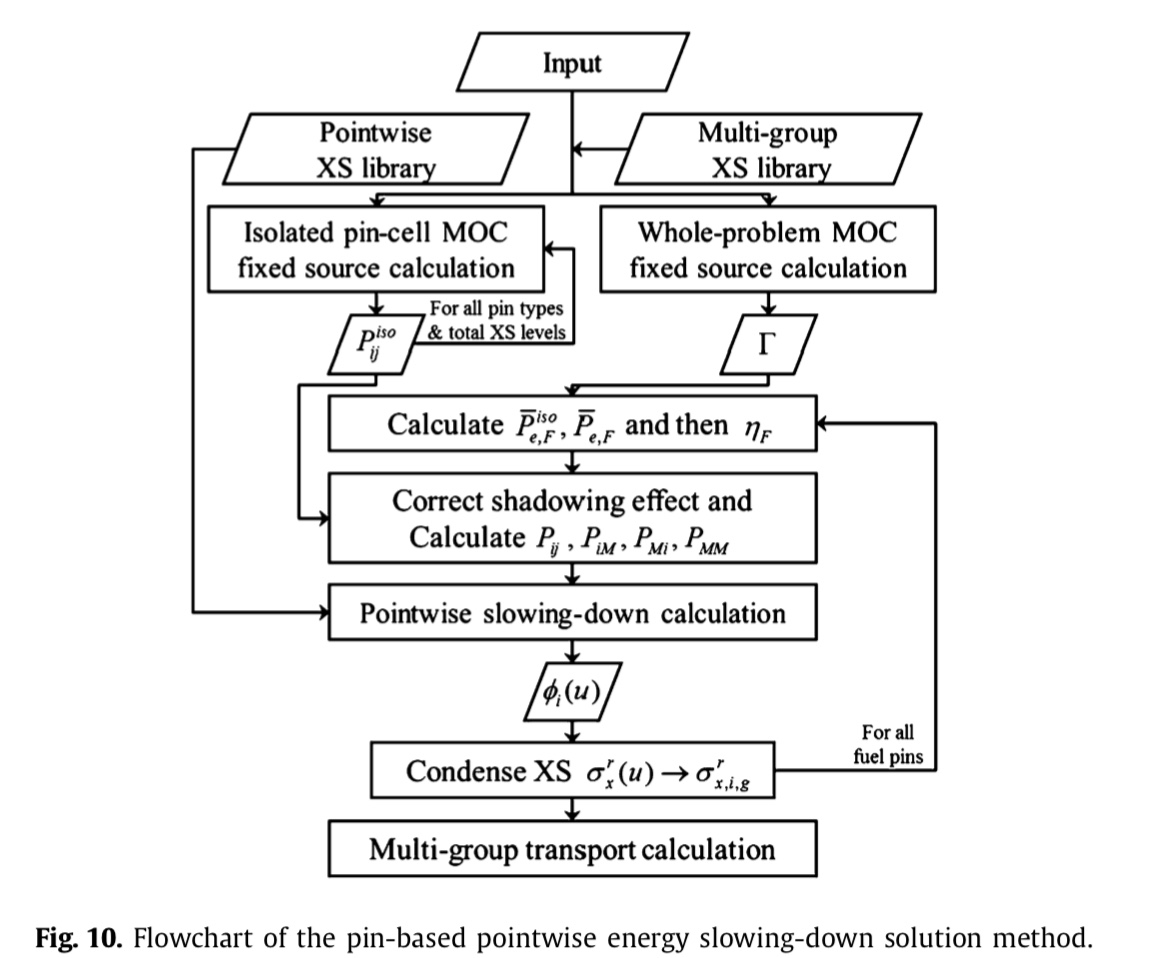
\includegraphics[width=0.65\linewidth]{fig10.jpeg}}
\end{frame}

\begin{frame}{Verification}{base pin problem}
\centering
\fcolorbox{fall}{white}{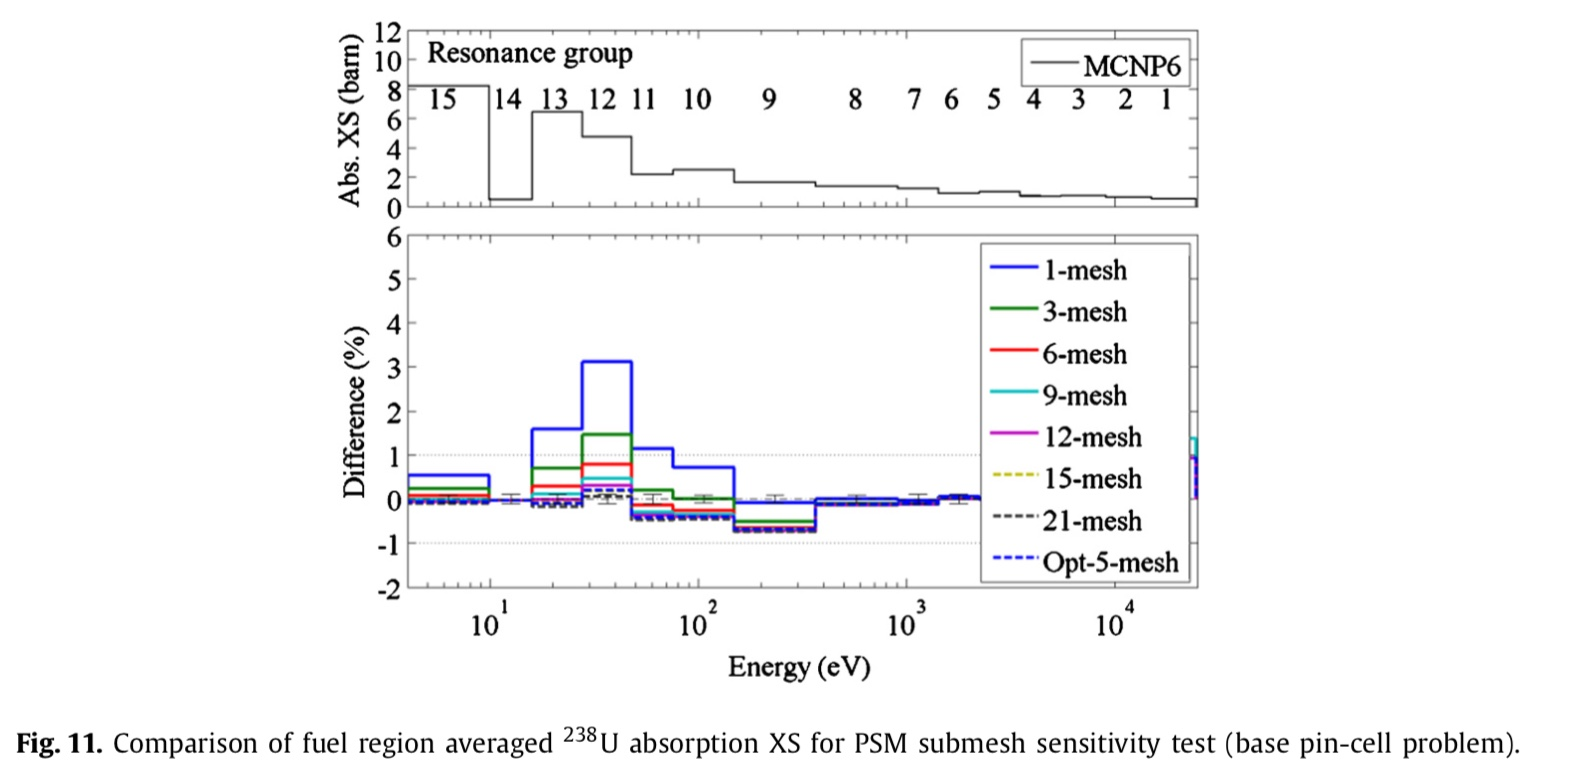
\includegraphics[width=0.85\linewidth]{fig11.jpeg}}
\end{frame}

\begin{frame}{Verification}{base pin problem}
\centering
\fcolorbox{fall}{white}{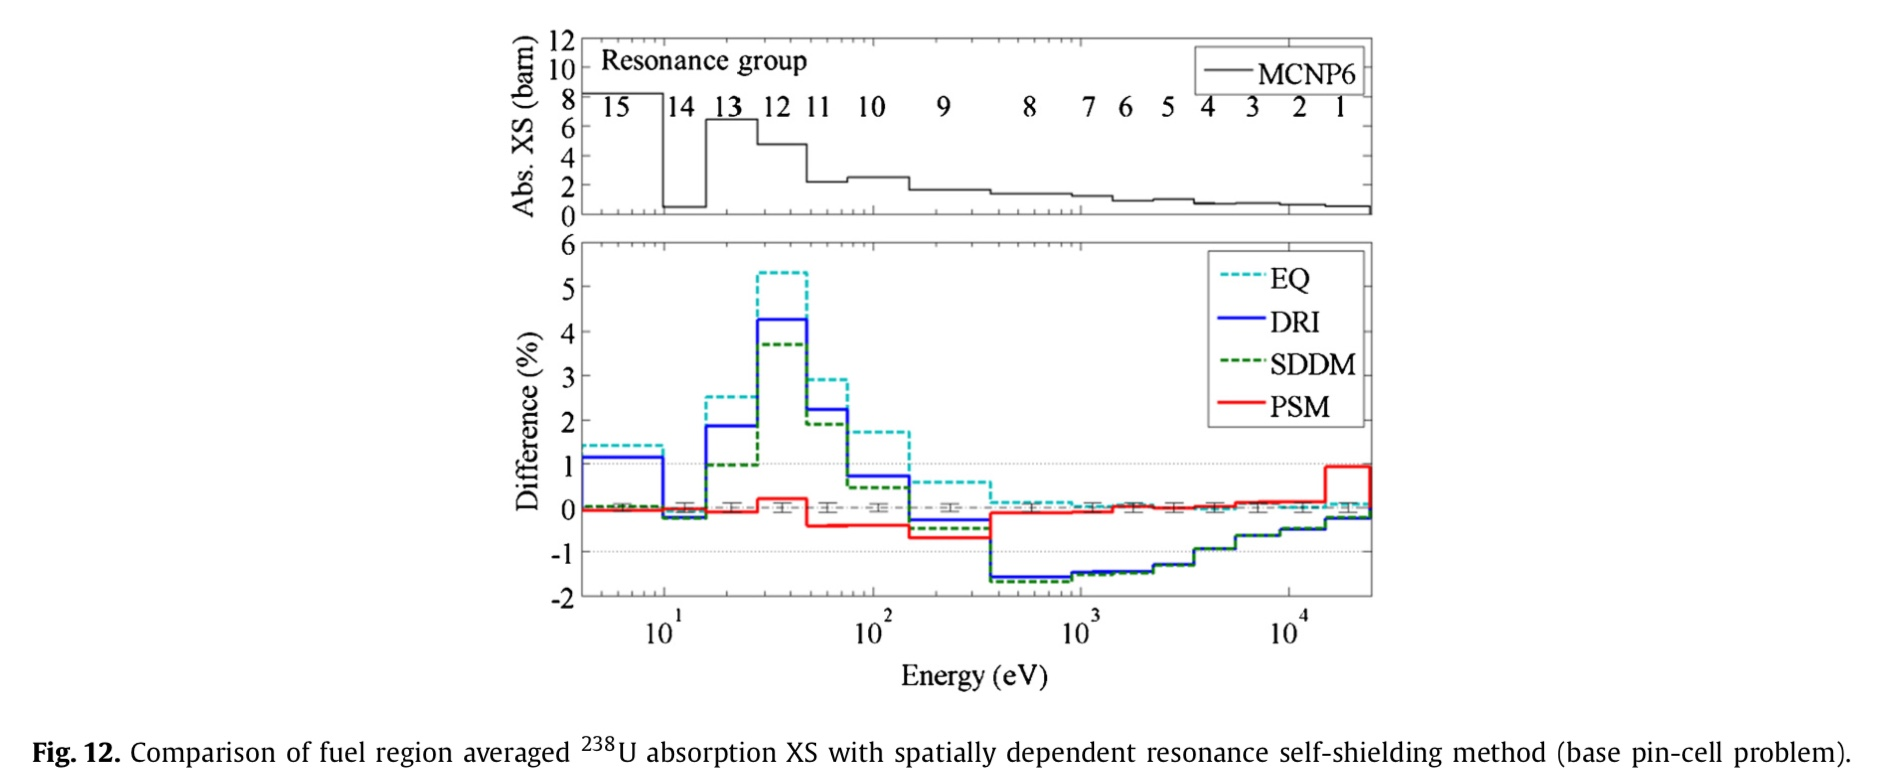
\includegraphics[width=0.85\linewidth]{fig12.jpeg}}
\end{frame}

\begin{frame}{Verification}{base pin problem}
\centering
\fcolorbox{fall}{white}{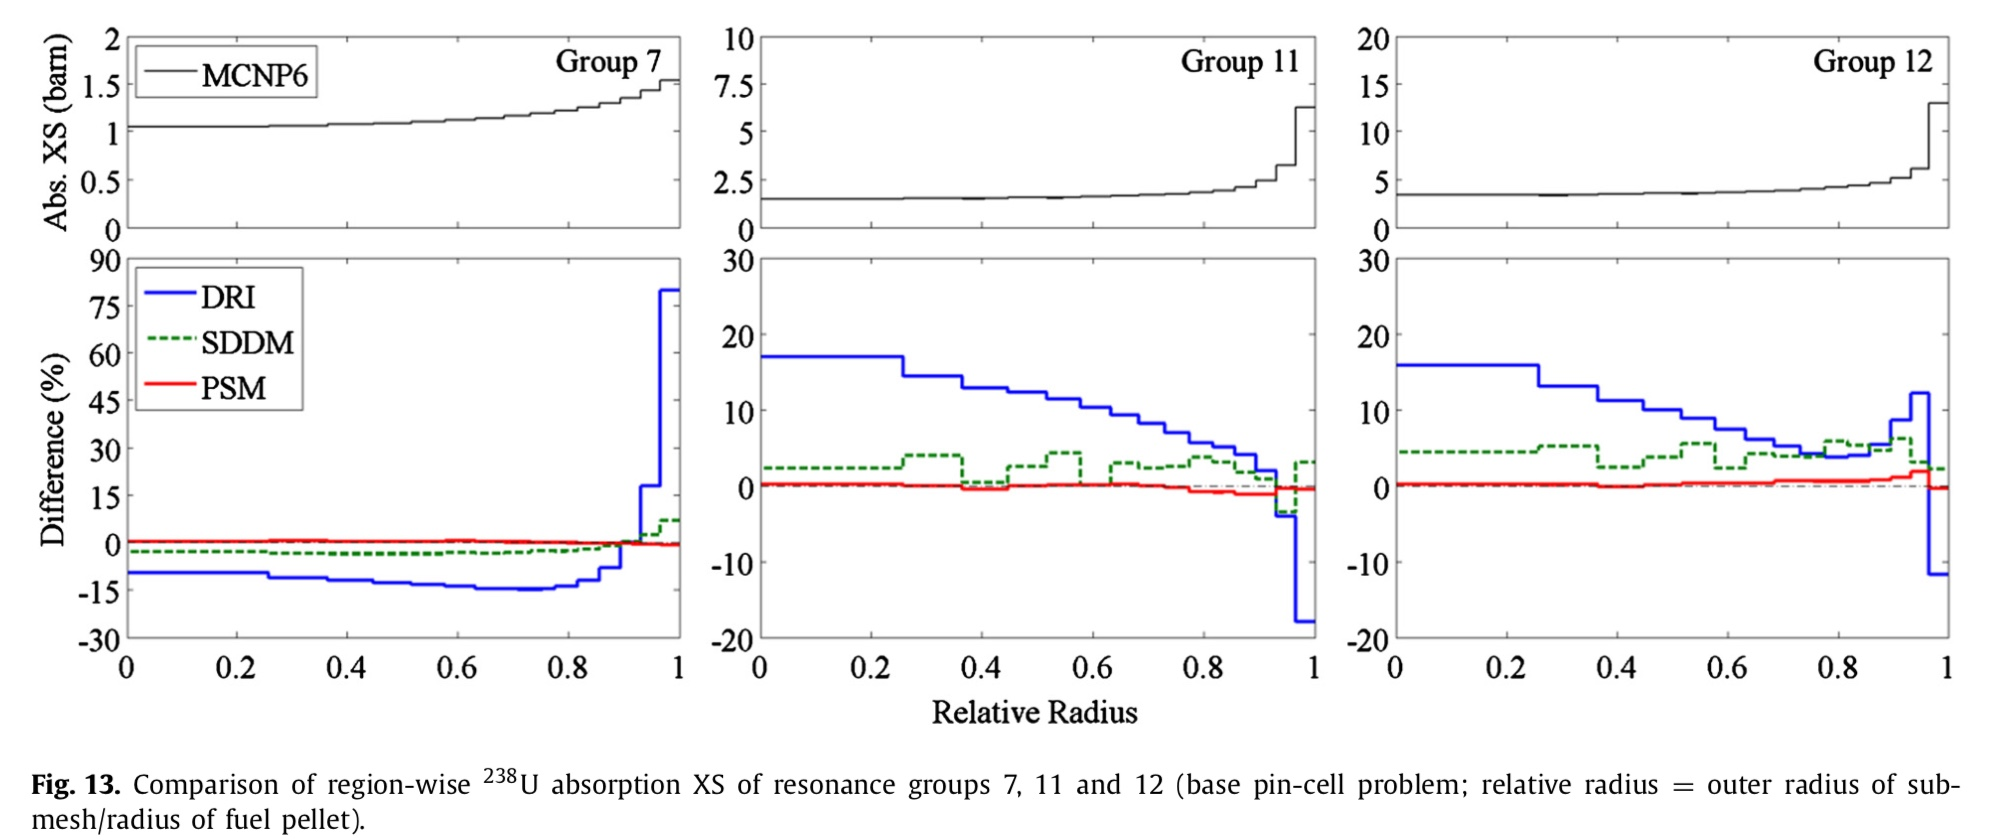
\includegraphics[width=0.85\linewidth]{fig13.jpeg}}
\end{frame}

\begin{frame}{Verification}{additional tests}
\centering
\fcolorbox{fall}{white}{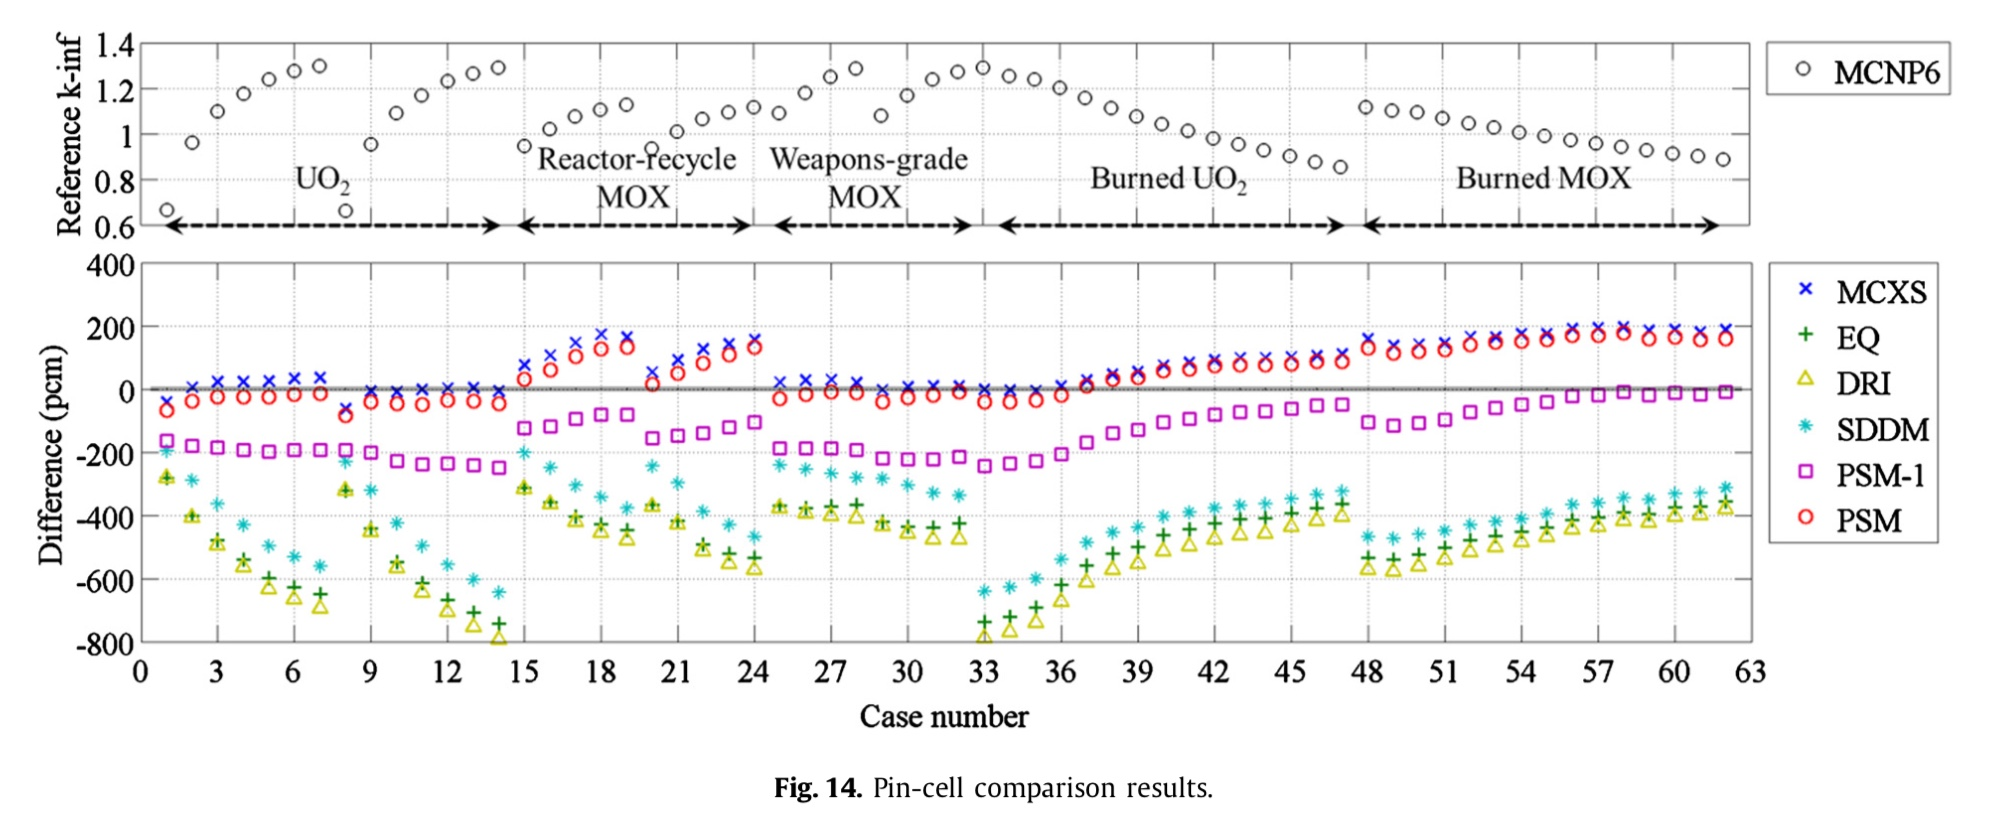
\includegraphics[width=0.85\linewidth]{fig14.jpeg}}
\end{frame}

\begin{frame}{Verification}{additional tests}
\centering
\fcolorbox{fall}{white}{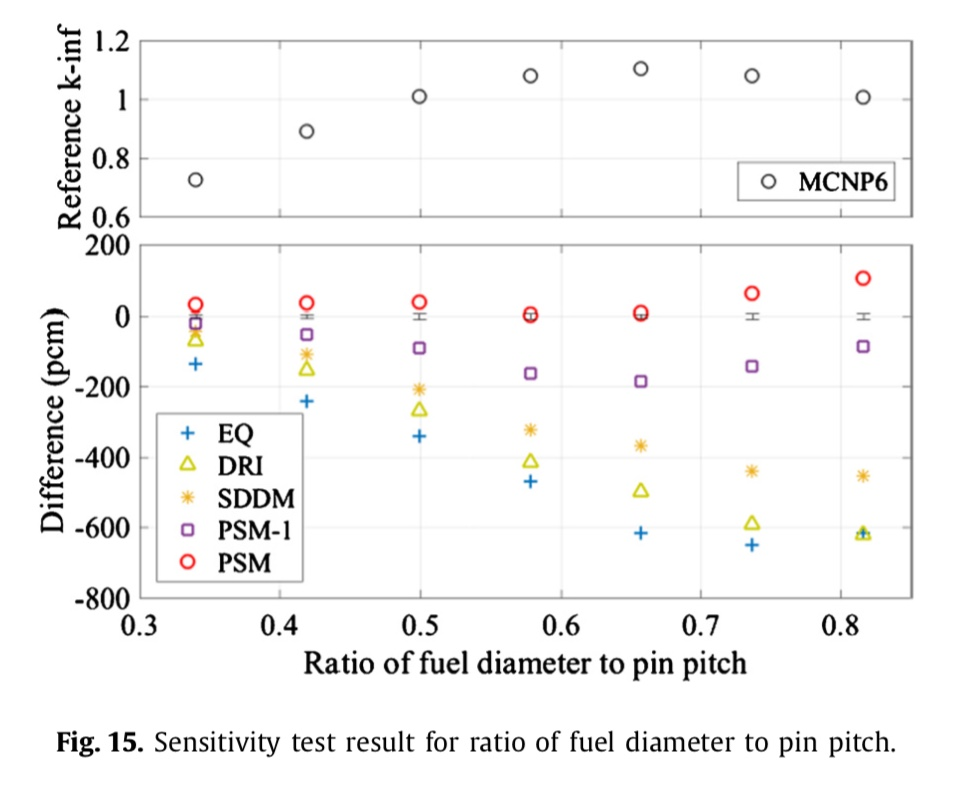
\includegraphics[width=0.55\linewidth]{fig15.jpeg}}
\end{frame}

\begin{frame}{Verification}{additional tests}
\centering
\fcolorbox{fall}{white}{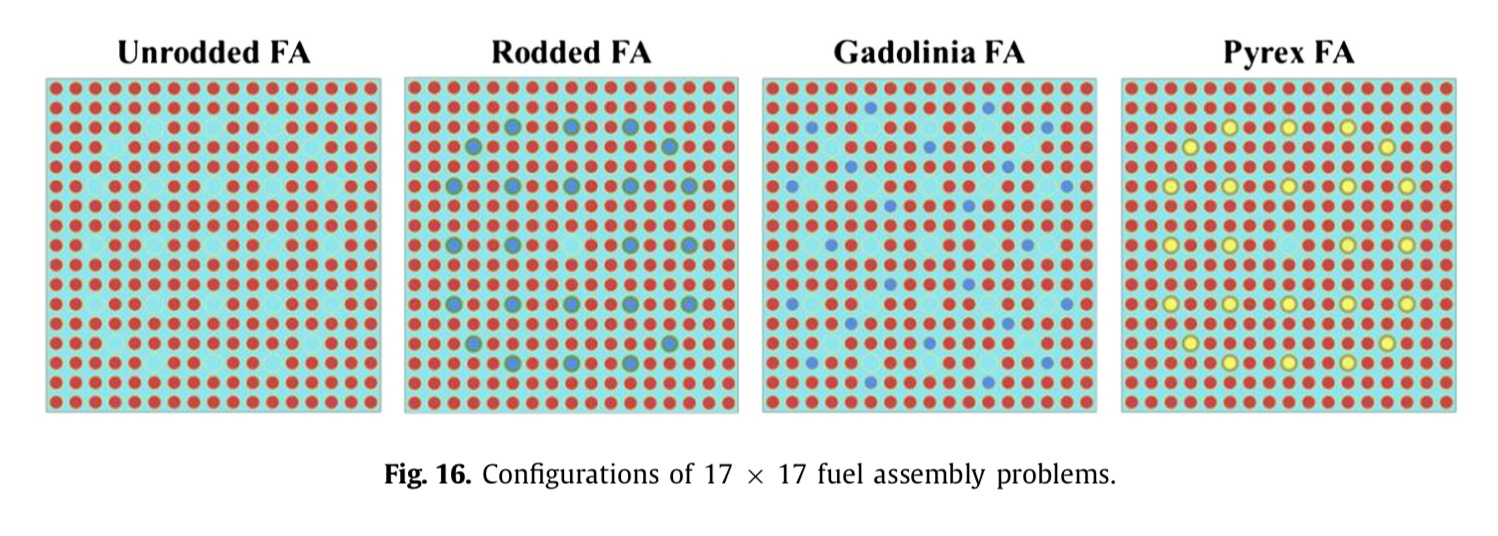
\includegraphics[width=0.85\linewidth]{fig16.jpeg}}
\end{frame}

\begin{frame}{Verification}{additional tests}
\centering
\fcolorbox{fall}{white}{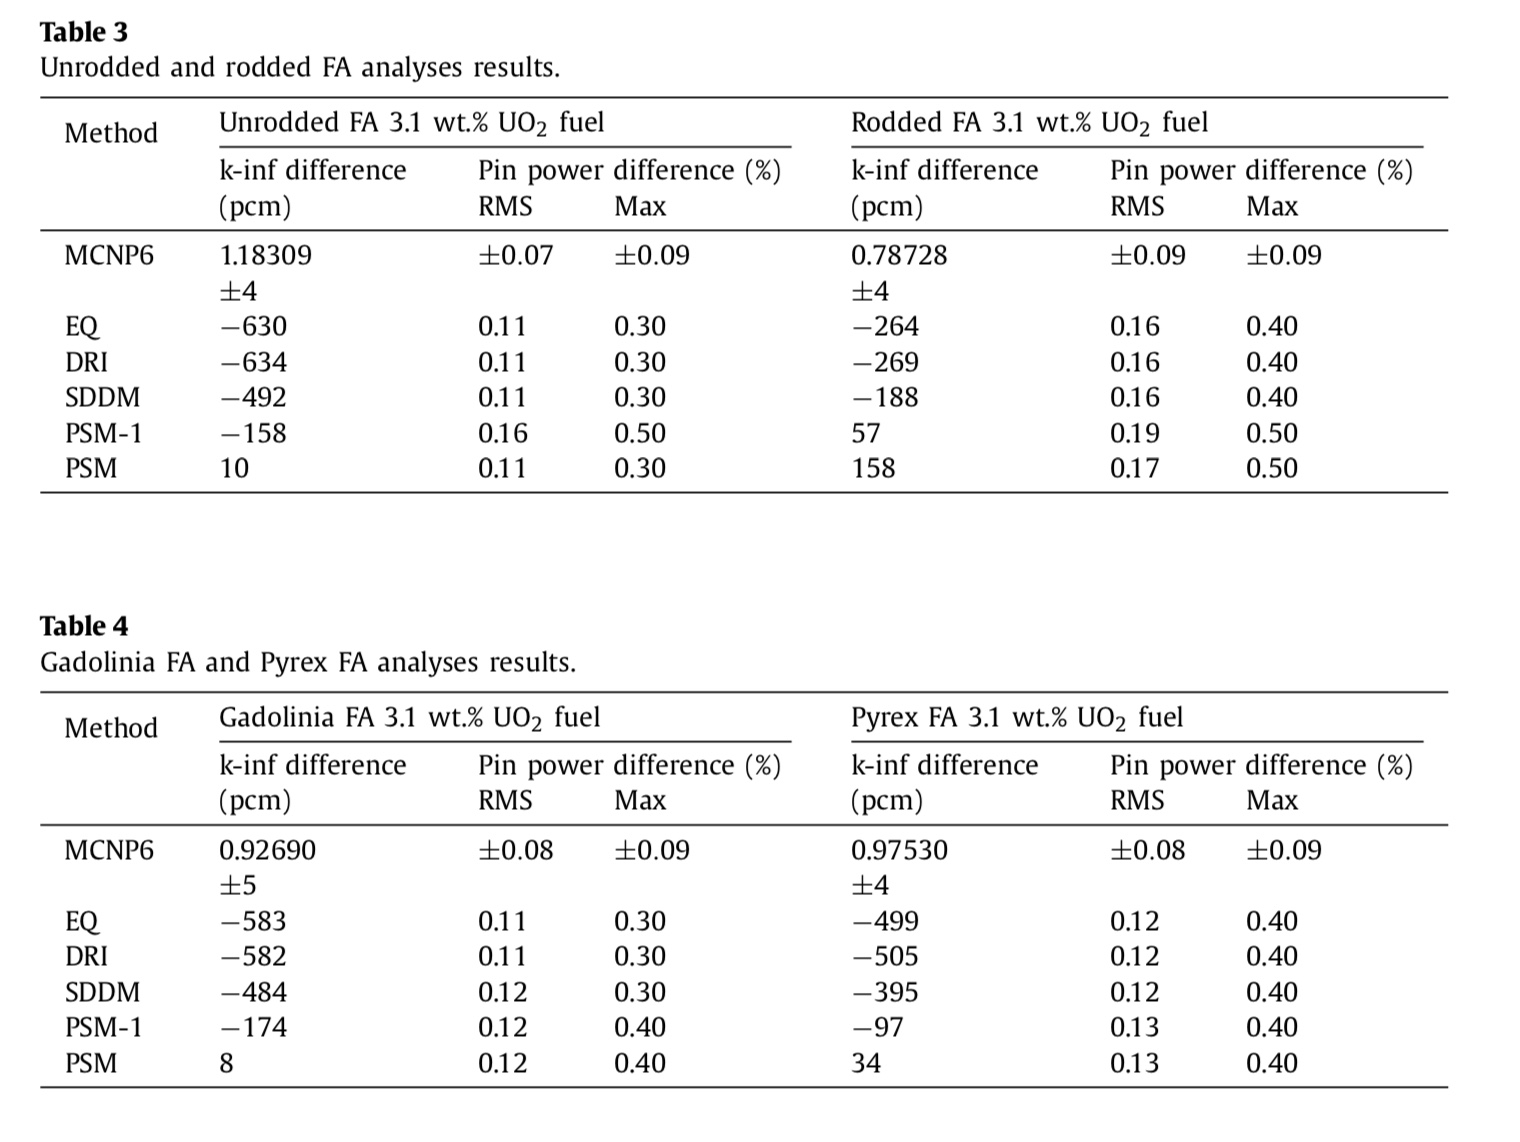
\includegraphics[width=0.6\linewidth]{tab3-4.jpeg}}
\end{frame}

\begin{frame}{Comparison of Computing Time}
\centering
\fcolorbox{fall}{white}{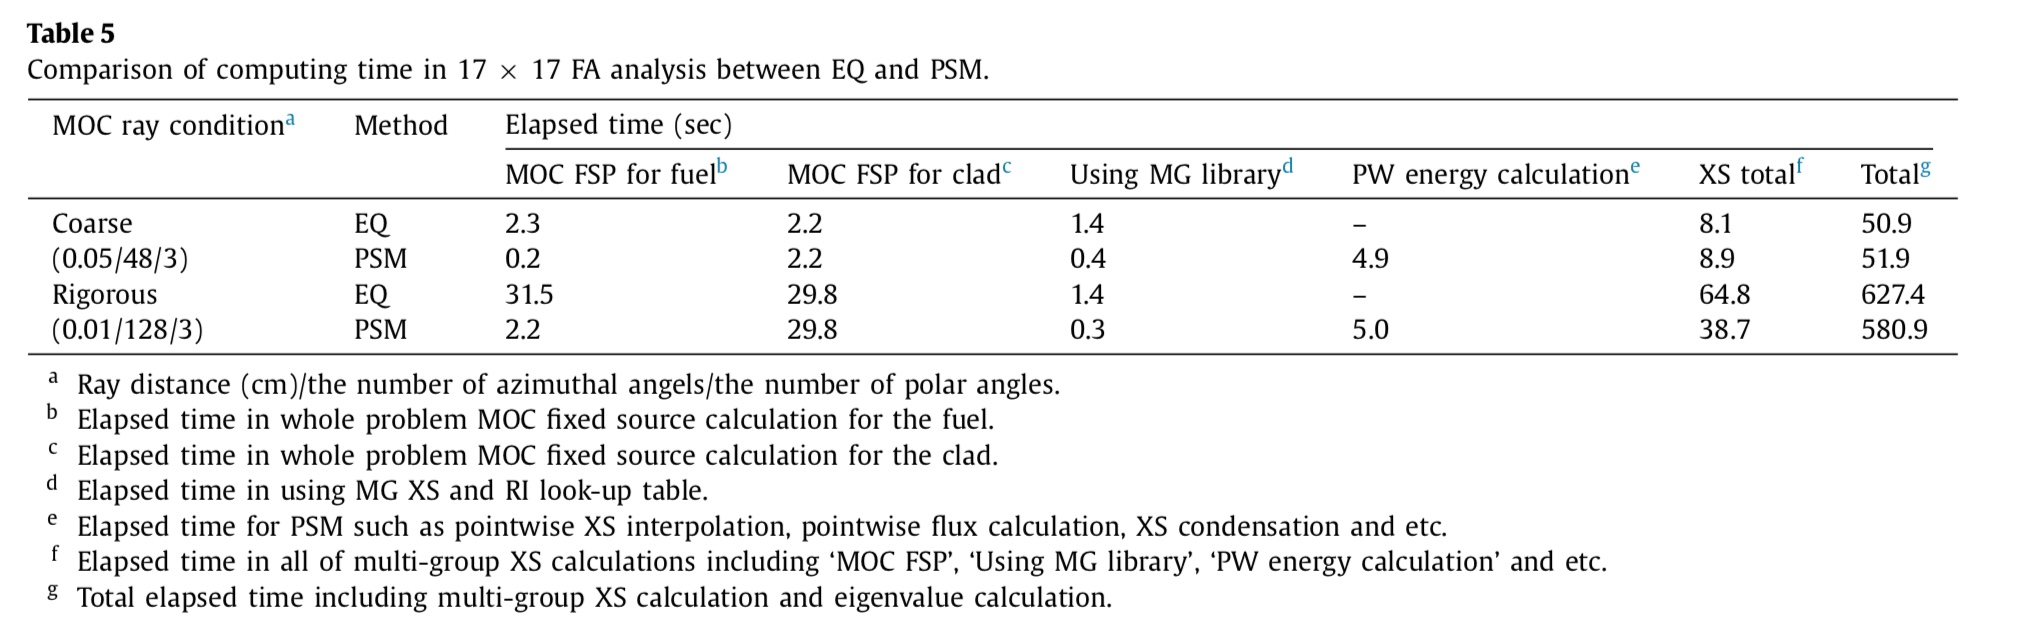
\includegraphics[width=0.9\linewidth]{table5.jpeg}}
\end{frame}

\begin{frame}{Conclusions}
\begin{itemize}
\item PSM eliminates the limitations of conventional equivalence methods.
\item Spatially dependent pointwise energy slowing down equation
\item Shadowing effect correction factors
\item Good agreement of PSM with MCNP6 (< 100 pcm) and 1\% difference in absorption XSs
\end{itemize}
\end{frame}

%slide
\begin{frame}
\centering
\Huge
Thanks! \\
Questions?
\end{frame}


\end{document}
